\documentclass[11pt,a4paper]{article}
% ---------------------------------------------------------------
% Preamble — biên dịch bằng XeLaTeX (tectonic)
% ---------------------------------------------------------------
\usepackage{fontspec}
\usepackage{unicode-math}

% Font chính: CM Unicode (phủ đủ dấu tiếng Việt). Nếu không có, đổi sang
% \setmainfont{Times New Roman} hoặc \setmainfont{Arial Unicode}.
\IfFontExistsTF{cmunrm.otf}{%
  \setmainfont{cmun}[
    Extension      = .otf,
    UprightFont    = *rm,
    BoldFont       = *bx,
    ItalicFont     = *ti,
    BoldItalicFont = *bi,
    Ligatures      = TeX ]
  \setmonofont{cmun}[
    Extension      = .otf,
    UprightFont    = *tt,
    BoldFont       = *tb,
    ItalicFont     = *it,
    Scale          = 0.92 ]
}{%
  \setmainfont{Times New Roman}[Ligatures=TeX]
  \setmonofont{Menlo}[Scale=0.85]
}

\usepackage[a4paper,top=2.5cm,bottom=2.5cm,left=2.6cm,right=2.6cm]{geometry}
\usepackage{amsmath}
\usepackage{graphicx}
\usepackage{float}
\usepackage{xcolor}
\usepackage{booktabs}
\usepackage{longtable}
\usepackage{tabularx}
\usepackage{array}
\usepackage{multirow}
\usepackage{enumitem}
\usepackage{caption}
\usepackage{subcaption}
\usepackage{listings}
\usepackage{fancyvrb}
\usepackage{fvextra}
\usepackage{fancyhdr}
\usepackage{titlesec}
\usepackage[most]{tcolorbox}
\usepackage[hidelinks,bookmarksnumbered]{hyperref}

% --------------------------- màu sắc ---------------------------
\definecolor{accent}{HTML}{1F4E79}
\definecolor{softbg}{HTML}{F3F6FA}
\definecolor{softbd}{HTML}{9DB8D4}
\definecolor{warmbg}{HTML}{FDF2E3}
\definecolor{warmbd}{HTML}{E0A458}
\definecolor{coolbg}{HTML}{EAF5EF}
\definecolor{coolbd}{HTML}{5CA184}
\definecolor{rulegray}{HTML}{BBBBBB}
\definecolor{codebg}{HTML}{F7F7F7}

% --------------------------- tiêu đề ---------------------------
\titleformat{\section}{\Large\bfseries\color{accent}}{\thesection.}{0.5em}{}
\titleformat{\subsection}{\large\bfseries}{\thesubsection}{0.5em}{}
\titlespacing*{\section}{0pt}{1.4em}{0.7em}
\titlespacing*{\subsection}{0pt}{1.1em}{0.5em}

\pagestyle{fancy}
\fancyhf{}
\fancyfoot[C]{\small\thepage}
\renewcommand{\headrulewidth}{0pt}

% --------------------------- bảng ------------------------------
\newcolumntype{L}[1]{>{\raggedright\arraybackslash}p{#1}}
\newcolumntype{C}[1]{>{\centering\arraybackslash}p{#1}}
\newcolumntype{R}[1]{>{\raggedleft\arraybackslash}p{#1}}
\newcolumntype{Y}{>{\raggedright\arraybackslash}X}
\renewcommand{\arraystretch}{1.18}
\captionsetup[table]{font=small,labelfont=bf,skip=4pt}
\captionsetup[figure]{font=small,labelfont=bf,skip=4pt}
\renewcommand{\tablename}{Bảng}
\renewcommand{\figurename}{Hình}
\renewcommand{\contentsname}{Mục lục}

% --------------------------- hộp nhấn mạnh ---------------------
\newtcolorbox{softbox}[1][]{
  colback=softbg, colframe=softbd, boxrule=0.6pt, arc=2pt,
  left=8pt, right=8pt, top=6pt, bottom=6pt, #1}
\newtcolorbox{warmbox}[1][]{
  colback=warmbg, colframe=warmbd, boxrule=0.6pt, arc=2pt,
  left=8pt, right=8pt, top=6pt, bottom=6pt, #1}
\newtcolorbox{coolbox}[1][]{
  colback=coolbg, colframe=coolbd, boxrule=0.6pt, arc=2pt,
  left=8pt, right=8pt, top=6pt, bottom=6pt, #1}
\newtcolorbox{plainbox}[1][]{
  colback=white, colframe=black, boxrule=0.5pt, arc=1pt,
  left=8pt, right=8pt, top=6pt, bottom=6pt, #1}

% --------------------------- code ------------------------------
\lstdefinestyle{plain}{
  basicstyle=\ttfamily\scriptsize,
  breaklines=true,
  breakatwhitespace=false,
  columns=fullflexible,
  keepspaces=true,
  showstringspaces=false,
  backgroundcolor=\color{codebg},
  frame=single,
  rulecolor=\color{rulegray},
  framesep=4pt,
  xleftmargin=6pt,
  xrightmargin=2pt,
  numbers=none,
  upquote=true,
  extendedchars=true,
  % Không dùng `literate`: XeTeX xử lý UTF-8 trực tiếp, cmuntt phủ đủ dấu tiếng Việt.
}
\lstset{style=plain}

% listings không xử lý đúng ký tự UTF-8 3 byte (ộ, ữ, ệ...). Mọi tệp mã nguồn
% có tiếng Việt được nạp bằng fvextra/fancyvrb — XeTeX đọc UTF-8 trực tiếp.
\newcommand{\srcfile}[2][]{%
  \VerbatimInput[fontsize=\scriptsize, frame=single, framesep=4pt,
    rulecolor=\color{rulegray}, breaklines, breakanywhere,
    breaksymbolleft={}, breaksymbolright={}, #1]{#2}}

% --------------------------- tiện ích --------------------------
\newcommand{\kpi}[2]{%
  \begin{minipage}[t]{0.24\linewidth}\centering
    {\large\bfseries #1}\\[2pt]{\footnotesize #2}
  \end{minipage}}
\newcommand{\req}{\textsuperscript{\textcolor{accent}{\scriptsize[BẮT BUỘC]}}}
\setlist[itemize]{leftmargin=1.4em,itemsep=2pt,topsep=3pt}
\setlist[enumerate]{leftmargin=1.7em,itemsep=2pt,topsep=3pt}

% --------------------------- bổ sung cho A4–A5 --------------------
\usepackage{multirow}
\usepackage{pdflscape}
\newcommand{\code}[1]{\texttt{\small #1}}
% Bảng dài dùng chung một kiểu chữ nhỏ
\newcommand{\smalltable}{\small}

% --------------------------- bổ sung cho A7 --------------------
\usepackage{tikz}
\usetikzlibrary{arrows.meta,positioning,fit,calc,backgrounds}
\tikzset{
  op/.style={draw, rounded corners=2pt, minimum height=5.5mm, minimum width=9mm,
             font=\scriptsize\ttfamily, fill=white},
  var/.style={font=\small, inner sep=1pt},
  flow/.style={-{Stealth[length=4pt]}, semithick},
}
\definecolor{rnncol}{HTML}{C8553D}
\definecolor{lstmcol}{HTML}{2E6F95}

\newcommand{\nDocs}{35}
\newcommand{\nDocsVi}{13}
\newcommand{\nDocsEn}{22}
\newcommand{\nHtmlVi}{10}
\newcommand{\nHtmlEn}{18}
\newcommand{\nPdfVi}{3}
\newcommand{\nPdfEn}{4}
\newcommand{\nPublishers}{16}
\newcommand{\nChunks}{424}
\newcommand{\nChunksVi}{273}
\newcommand{\nChunksEn}{151}
\newcommand{\tokMean}{337}
\newcommand{\tokMin}{63}
\newcommand{\tokMax}{400}
\newcommand{\nQuestions}{30}
\newcommand{\nInScope}{26}
\newcommand{\nOos}{4}
\newcommand{\nQEn}{4}
\newcommand{\nGoldPairs}{269}
\newcommand{\goldMin}{2}
\newcommand{\goldMax}{21}
\newcommand{\poolMean}{48}
\newcommand{\relAgree}{12/15}
\newcommand{\relAgreeLenient}{15--17/25}
\newcommand{\claimAgree}{5/5}
\newcommand{\nFacts}{1.779}
\newcommand{\nBilingualFacts}{52}
\newcommand{\nProposed}{2.195}
\newcommand{\nAccepted}{2.124}
\newcommand{\nRejQuote}{60}
\newcommand{\nRejOther}{11}
\newcommand{\extractTokens}{522.949}
\newcommand{\nNodes}{2.846}
\newcommand{\nRels}{5.027}
\newcommand{\nSupportedBy}{2.116}
\newcommand{\nRowsStatus}{686.019}
\newcommand{\nProfilesStatus}{634.636}
\newcommand{\nRowsType}{22.027}
\newcommand{\nFeatures}{19}
\newcommand{\trainSeconds}{66}
\newcommand{\predictMs}{0,033}
\newcommand{\tempStatus}{0,819}
\newcommand{\tempType}{0,612}
\newcommand{\eceStatusBefore}{0,1116}
\newcommand{\eceStatusAfter}{0,0881}
\newcommand{\eceTypeBefore}{0,0962}
\newcommand{\eceTypeAfter}{0,0425}
\newcommand{\eceStatusPrior}{0,0056}
\newcommand{\eceTypePrior}{0,0237}
\newcommand{\bestEpochStatus}{5}
\newcommand{\epochsStatus}{13}
\newcommand{\bestEpochType}{11}
\newcommand{\epochsType}{19}
\newcommand{\preTP}{524}
\newcommand{\preSupport}{2.295}
\newcommand{\prePrecision}{0,0357}
\newcommand{\typeOneTP}{149}
\newcommand{\typeOneSupport}{298}
\newcommand{\typeOnePred}{875}
\newcommand{\typeOnePrecision}{0,1703}
\newcommand{\answeredZero}{24/26}
\newcommand{\answeredTwo}{25/26}
\newcommand{\supportedZero}{98,9\%}
\newcommand{\supportedTwo}{97,9\%}
\newcommand{\unsupportedZero}{0,6\%}
\newcommand{\unsupportedTwo}{0,0\%}
\newcommand{\claimsZero}{175}
\newcommand{\claimsTwo}{186}
\newcommand{\refusalOos}{100\%}
\newcommand{\falseRefusalTwo}{3,9\%}
\newcommand{\falseRefusalZero}{7,7\%}
\newcommand{\latencyP}{2,46}
\newcommand{\latencyMax}{8,82}
\newcommand{\vZeroUnsupported}{39,1\%}
\newcommand{\vOneUnsupported}{4,0\%}
\newcommand{\vOneFalseRefusal}{19,2\%}
\newcommand{\gxAdded}{51}
\newcommand{\gxRelevant}{17,6\%}
\newcommand{\gxOther}{39,2\%}
\newcommand{\gxOutside}{96,1\%}
\newcommand{\gxNew}{7}
\newcommand{\llmModel}{gemma-4}
\newcommand{\uiFirstTextP}{2,9}
\newcommand{\rrfK}{60}
\newcommand{\expandN}{2}
\newcommand{\oosMin}{0,78}
\newcommand{\embedDim}{1.024}
\newcommand{\nPrevalenceOther}{361.959}
\newcommand{\yFifteencA}{213.703}
\newcommand{\yFifteencB}{4.631}
\newcommand{\yFifteencC}{35.346}
\newcommand{\yFifteentotal}{253.680}
\newcommand{\yTwentyThreecA}{361.959}
\newcommand{\yTwentyThreecB}{10.594}
\newcommand{\yTwentyThreecC}{59.786}
\newcommand{\yTwentyThreetotal}{432.339}
\newcommand{\typeCountB}{1.958}
\newcommand{\typeCountC}{20.069}

\newcommand{\chosenStatus}{CNN-1D}
\newcommand{\rowsStatus}{686.019}
\newcommand{\dlTempStatus}{0,778}
\newcommand{\chosenType}{LSTM}
\newcommand{\rowsType}{22.027}
\newcommand{\dlTempType}{0,407}
\newcommand{\trainRatio}{56}
\newcommand{\dlTotalMin}{59}
\newcommand{\dlSeeds}{3}
\newcommand{\intentN}{22}
\newcommand{\intentOk}{22}
\newcommand{\intakeLlm}{93\%}
\newcommand{\intakeLlmOk}{39/42}
\newcommand{\intakeRules}{83\%}
\newcommand{\intakeRulesOk}{35/42}
\newcommand{\intakeMerged}{98\%}
\newcommand{\intakeMergedOk}{41/42}
\newcommand{\vOneIntakeLlm}{38\%}
\newcommand{\vOneIntakeRules}{86\%}
\newcommand{\vOneIntakeMerged}{95\%}
\newcommand{\intakeFields}{42}
\newcommand{\intakeMsgs}{8}
\newcommand{\safetyN}{11}
\newcommand{\safetyMulti}{11/11}
\newcommand{\safetySingle}{11/11}
\newcommand{\convMaRisk}{4/4}
\newcommand{\convMaFields}{28/28}
\newcommand{\convMaCites}{10,0}
\newcommand{\convMaCalls}{18}
\newcommand{\convMaSecs}{21}
\newcommand{\convSaRisk}{4/4}
\newcommand{\convSaFields}{21/28}
\newcommand{\convSaCites}{5,5}
\newcommand{\convSaCalls}{19}
\newcommand{\convSaSecs}{27}
\newcommand{\convN}{4}
\newcommand{\saAgeErr}{3}
\newcommand{\saGenErr}{4}
\newcommand{\vOneConvRisk}{3/4}
\newcommand{\vOneConvFields}{26/28}

\makeatletter
\newcommand{\tablerows}[1]{\@@input #1 }
\makeatother

\hypersetup{pdftitle={Diabeque — Hệ đa agent cho chẩn đoán và tư vấn bệnh tiểu đường}, pdfauthor={Nhóm 02}}

\tikzset{
  box/.style={draw=softbd, fill=softbg, rounded corners=2pt, align=center, font=\footnotesize, minimum height=1.0cm, text width=2.6cm},
  agent/.style={draw=accent, fill=softbg, rounded corners=3pt, align=center, font=\footnotesize, minimum height=1.0cm, text width=2.55cm},
  guard/.style={draw=warmbd, fill=warmbg, rounded corners=3pt, align=center, font=\footnotesize, minimum height=1.0cm, text width=2.6cm},
  arr/.style={-{Stealth[length=2mm]}, draw=accent!80!black},
  lab/.style={font=\scriptsize\ttfamily, fill=white, inner sep=1pt}}

\begin{document}

% ==================================================================
\thispagestyle{empty}
\begin{center}
  \vspace*{1.0cm}
  {\large\scshape Học viện Công nghệ Bưu chính Viễn thông}\\[4pt]
  {\normalsize Khoa Công nghệ Thông tin}\\[10pt]
  \rule{0.35\linewidth}{0.4pt}\\[14pt]
  {\normalsize Intelligent System Development — Tiểu luận Final, phần Project}\\[22pt]
  \includegraphics[width=2.6cm]{../assets/diabeque-mark.pdf}\\[6pt]
  {\Huge\bfseries Diabeque}\\[10pt]
  {\large Hệ đa agent cho chẩn đoán và tư vấn bệnh tiểu đường}\\[32pt]
  {\large\bfseries Nhóm 02}\\[6pt]
  {\small Trần Xuân Thành — B23DCAT280 — E23CNPM01}\\[4pt]
  {\small Giảng viên hướng dẫn: Dinh Que Tran, Ph.D., Assoc. Prof.}\\[22pt]
  {\small Học kỳ I.2026}
\end{center}

\vspace{0.6cm}
\begin{center}\bfseries Tóm tắt\end{center}
\begin{quote}\small
Diabeque là trợ lý hội thoại gồm sáu agent phối hợp theo mẫu điều phối--chuyên gia trên LangGraph: an toàn đầu vào,
điều phối, thu thập thông tin, dự đoán nguy cơ, tra cứu tri thức, tư vấn, và một lớp an toàn đầu ra. Agent dự đoán dùng
mô hình học sâu huấn luyện trên \nRowsStatus{} bản ghi khảo sát BRFSS; ba kiến trúc MLP, CNN-1D và LSTM được so sánh
với \dlSeeds{} seed, và mô hình được chọn theo macro-F1 tập xác thực (\chosenStatus{} cho bài ba nhóm, \chosenType{} cho bài
Type 1/2). Agent tra cứu dùng lại kho tri thức \texttt{KB\_diabet} (\nDocs{} tài liệu từ link và PDF) và pipeline RAG có cổng
trích dẫn. Trên bộ kịch bản viết tay, hệ thống phân loại đúng \intentOk/\intentN{} ý định, trích đúng \intakeMergedOk{}
trường hồ sơ, xử lý đúng \safetyMulti{} tình huống an toàn, và đưa vào mô hình đúng \convMaFields{} trường hồ sơ, so với
\convSaFields{} của một agent duy nhất dùng cùng mô hình ngôn ngữ và cùng công cụ. Hệ thống ước lượng nguy cơ, không chẩn
đoán.
\end{quote}

\newpage
\tableofcontents
\newpage

% ==================================================================
\section{Giới thiệu}

\subsection{Bài toán}

Đái tháo đường típ 2 tiến triển âm thầm: nhiều người có tiền đái tháo đường hoặc đã mắc bệnh mà không biết. Sàng lọc sớm
dựa trên các yếu tố nguy cơ dễ hỏi (tuổi, BMI, huyết áp, mỡ máu, vận động) giúp xác định ai nên đi xét nghiệm. Sau khi biết
nguy cơ, người dùng cần lời khuyên cụ thể và đáng tin cậy, nghĩa là mỗi lời khuyên phải chỉ được về một tài liệu y tế.

Hai năng lực này đã có ở các bài trước: bộ phân loại khảo sát BRFSS (Chương 1--2 của tiểu luận, A8) và pipeline RAG có trích
dẫn (Chương 5). Mỗi thành phần chạy riêng: bộ phân loại cần người dùng điền đủ một biểu mẫu 19 trường, còn RAG trả lời
từng câu hỏi độc lập. Project ghép chúng thành một trợ lý hội thoại: người dùng nói bằng lời thường, hệ thống tự quyết định
cần hỏi thêm gì, khi nào dự đoán, khi nào tra cứu, và chặn những câu trả lời không an toàn.

\subsection{Phạm vi: sàng lọc, không chẩn đoán}

Đề tài ghi “chẩn đoán và tư vấn”. Chẩn đoán đái tháo đường cần xét nghiệm đường huyết lúc đói, HbA1c hoặc nghiệm pháp dung
nạp glucose. Dữ liệu BRFSS là câu trả lời tự báo cáo qua điện thoại, không có xét nghiệm. Vì vậy hệ thống hiểu “chẩn đoán”
theo nghĩa \emph{sàng lọc nguy cơ}: ước lượng tỷ lệ ở những người có hồ sơ tương tự, và khuyên đi xét nghiệm khi nguy cơ
cao. Hệ thống không kết luận một người mắc bệnh, không kê thuốc hay liều.

\subsection{Kết quả chính}

\begin{center}
\kpi{\intentOk/\intentN}{ý định được phân loại đúng}
\kpi{\intakeMerged}{trường hồ sơ được trích đúng}
\kpi{\safetyMulti}{tình huống an toàn xử lý đúng}
\kpi{\convMaFields}{trường đưa vào mô hình đúng (một agent: \convSaFields)}
\end{center}

\begin{table}[H]
\centering
\caption{Bảy mục của báo cáo và phần mã tương ứng}
\begin{tabularx}{\linewidth}{L{4.2cm}Y}
\toprule
Mục & Nội dung và mã \\
\midrule
2. Kiến trúc hệ đa agent & Sáu agent, trạng thái chung, đồ thị LangGraph, đánh giá so với một agent: \code{backend/app/agents/}, \code{eval/} \\
3. Data & BRFSS 2015 và 2023, kho tài liệu, bộ kịch bản đánh giá: \code{data/survey.db}, \code{eval/scenarios.yaml} \\
4. Deep learning cho Diabetes & MLP, CNN-1D, LSTM: \code{backend/app/nets.py}, \code{pipeline/train\_dl.py} \\
5. KB + RAG & Kho \code{KB\_diabet} trên Neo4j và pipeline RAG làm công cụ của agent: \code{retrieval.py}, \code{agents/tools.py} \\
6. Code\_Demo & API SSE, giao diện Next.js, kiểm thử: \code{backend/app/main.py}, \code{frontend/}, \code{tests/} \\
\bottomrule
\end{tabularx}
\end{table}

% ==================================================================
\section{Kiến trúc hệ đa agent}

\subsection{Tổng quan}

Hệ thống theo mẫu \emph{điều phối--chuyên gia} (supervisor): một agent điều phối đọc tin nhắn, xác định ý định và chuyển
cho agent chuyên môn. Hai lớp an toàn bọc ngoài: một lớp kiểm tin nhắn trước khi vào hệ thống, một lớp kiểm câu trả lời
trước khi gửi đi.

\begin{figure}[H]
\centering
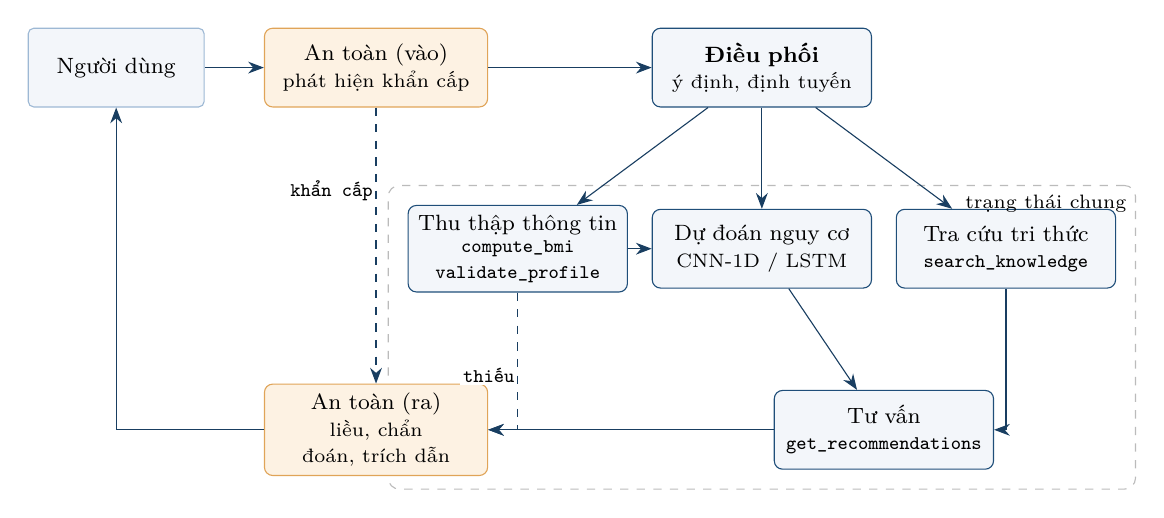
\begin{tikzpicture}
  \node[box, text width=2.0cm] (user) at (0,0) {Người dùng};
  \node[guard] (gin) at (3.3,0) {An toàn (vào)\\\scriptsize phát hiện khẩn cấp};
  \node[agent] (orch) at (8.2,0) {\textbf{Điều phối}\\\scriptsize ý định, định tuyến};
  \node[agent] (intake) at (5.1,-2.3) {Thu thập thông tin\\\scriptsize\ttfamily compute\_bmi\\validate\_profile};
  \node[agent] (risk) at (8.2,-2.3) {Dự đoán nguy cơ\\\scriptsize \chosenStatus{} / \chosenType};
  \node[agent] (kb) at (11.3,-2.3) {Tra cứu tri thức\\\scriptsize\ttfamily search\_knowledge};
  \node[agent] (adv) at (9.75,-4.6) {Tư vấn\\\scriptsize\ttfamily get\_recommendations};
  \node[guard] (gout) at (3.3,-4.6) {An toàn (ra)\\\scriptsize liều, chẩn đoán, trích dẫn};
  \begin{scope}[on background layer]
    \node[draw=rulegray, dashed, rounded corners, fit=(intake)(kb)(adv), inner sep=7pt] (st) {};
  \end{scope}
  \node[font=\scriptsize, anchor=north east] at (st.north east) {trạng thái chung};
  \draw[arr] (user) -- (gin);
  \draw[arr] (gin) -- (orch);
  \draw[arr] (orch) -- (intake);
  \draw[arr] (orch) -- (risk.north);
  \draw[arr] (orch) -- (kb);
  \draw[arr] (intake) -- (risk);
  \draw[arr] (risk) -- (adv);
  \draw[arr, dashed] (intake.south) |- node[lab, pos=0.3, left] {thiếu} (gout.east);
  \draw[arr] (kb) |- (adv.east);
  \draw[arr] (adv) -- (gout);
  \draw[arr] (gout.west) -| (user.south);
  \draw[arr, dashed] (gin) -- node[lab, left, pos=0.3] {khẩn cấp} (gout);
\end{tikzpicture}
\caption{Kiến trúc Diabeque. Thu thập chuyển sang dự đoán khi hồ sơ đủ; mũi tên nét đứt là các nhánh dừng sớm (hồ sơ còn thiếu, khẩn cấp).}
\label{fig:arch}
\end{figure}

\paragraph{Ba nhánh của một lượt.}
\begin{itemize}
  \item \textbf{Kiến thức}: điều phối $\to$ tra cứu tri thức $\to$ an toàn (ra).
  \item \textbf{Đánh giá nguy cơ}: điều phối $\to$ thu thập. Nếu hồ sơ còn thiếu, hệ thống hỏi thêm và kết thúc lượt; lượt sau
        người dùng trả lời, thu thập cập nhật hồ sơ. Khi đủ: dự đoán $\to$ tư vấn $\to$ an toàn (ra).
  \item \textbf{Khẩn cấp}: an toàn (vào) $\to$ an toàn (ra), không qua agent nào khác.
\end{itemize}
Chào hỏi và câu ngoài phạm vi được điều phối viên trả lời bằng văn bản cố định rồi đi thẳng tới an toàn (ra).

\subsection{Các agent}

\begin{table}[H]
\centering
\caption{Vai trò, cách ra quyết định và công cụ của từng agent}
\begin{tabularx}{\linewidth}{L{2.4cm}YL{3.4cm}}
\toprule
Agent & Việc làm & Cách làm \\
\midrule
An toàn (vào) & Phát hiện dấu hiệu cấp cứu: lú lẫn, bất tỉnh, khó thở, nôn nhiều, đường huyết $\geq 400$ mg/dL hoặc $< 70$ mg/dL. & Luật (biểu thức chính quy) \\
Điều phối & Xếp tin nhắn vào bốn ý định: \code{knowledge}, \code{assess\_risk}, \code{greeting}, \code{out\_of\_scope}. & LLM gọi công cụ \code{IntentDecision}; luật dự phòng khi LLM lỗi \\
Thu thập thông tin & Trích thông tin sức khỏe từ lời nói, đổi sang mã BRFSS, hỏi tối đa 3 câu mỗi lượt cho 7 trường bắt buộc. & LLM \code{IntakeExtraction} + luật; \code{compute\_bmi}, \code{validate\_profile} \\
Dự đoán nguy cơ & Gọi mô hình ba nhóm, hoặc mô hình Type 1/2 nếu người dùng nói đã được chẩn đoán; viết phần kết quả. & Mô hình học sâu (mục~\ref{sec:dl}); văn bản sinh bằng code \\
Tra cứu tri thức & Trả lời câu hỏi kiến thức có trích dẫn. & Pipeline RAG (mục~\ref{sec:kb}) \\
Tư vấn & Dựng truy vấn từ các yếu tố nguy cơ trong hồ sơ, lấy khuyến nghị có nguồn, viết 3--6 lời khuyên. & \code{get\_recommendations} + LLM + cổng trích dẫn \\
An toàn (ra) & Bỏ câu chứa liều thuốc hoặc kết luận chẩn đoán cá nhân; phần không còn trích dẫn bị thay bằng lời khuyên hỏi bác sĩ. & Luật \\
\bottomrule
\end{tabularx}
\end{table}

\paragraph{Nguyên tắc phân chia: LLM chỉ làm phần cần hiểu ngôn ngữ.}
Ba việc được giao cho LLM: hiểu ý định, trích thông tin từ câu nói tự do, và viết câu trả lời từ nguồn. Mọi việc có đáp án
xác định được viết bằng code: tính BMI, đổi tuổi sang nhóm tuổi BRFSS (18--24 là nhóm 1, mỗi nhóm 5 năm, 80 trở lên là
nhóm 13), kiểm miền giá trị, định dạng xác suất, và toàn bộ lớp an toàn. Mục~\ref{sec:eval} cho thấy lý do: khi giao việc đổi
nhóm tuổi cho LLM, một agent duy nhất làm sai \saAgeErr/\convN{} lần dù quy tắc có trong lời nhắc.

\paragraph{Thu thập: LLM và luật bổ sung cho nhau.}
Agent thu thập chạy hai bộ trích xuất trên cùng tin nhắn: LLM điền một lược đồ 15 trường (tuổi, giới, chiều cao, cân nặng,
các câu có/không), và một bộ luật nhận các cách nói phổ biến (“52 tuổi”, “1m65”, “80kg”, “huyết áp bình thường”, “ít vận
động”). Kết quả của LLM được ưu tiên; luật chỉ điền các trường LLM để trống. Bộ luật đọc phủ định theo từng vế: “huyết áp
cao và mỡ máu bình thường” cho huyết áp = có, mỡ máu = không; “huyết áp và mỡ máu bình thường” cho cả hai = không.

\paragraph{Dự đoán: hai cách đọc xác suất.}
Mô hình được huấn luyện với trọng số lớp tỷ lệ nghịch với tần suất để không bỏ sót các lớp ít mẫu, nên xác suất đầu ra bị
đẩy về phía lớp hiếm. Với trọng số $w_c \propto 1/n_c$, nhân xác suất với $n_c$ rồi chuẩn hóa sẽ đưa về tần suất của dữ liệu:
\[ \tilde p_c = \frac{p_c\, n_c}{\sum_k p_k\, n_k}. \]
A8 đo được ECE trên tập kiểm tra giảm từ 0,088 xuống 0,006 với phép hiệu chỉnh này. Giao diện hiển thị $\tilde p$ (“tỷ lệ ở
những người có hồ sơ tương tự”), còn nhãn của mô hình có trọng số được nêu riêng là kết quả “chế độ sàng lọc” và dùng để
chọn chủ đề tư vấn. Ví dụ hồ sơ nam 52 tuổi, BMI 29,4, huyết áp cao, ít vận động: mô hình có trọng số cho 57\% thuộc nhóm
“đã được thông báo mắc đái tháo đường”, sau hiệu chỉnh còn 35\%.

\subsection{Trạng thái chung và cài đặt bằng LangGraph}

Mọi agent đọc và ghi một đối tượng \code{SessionState} (\code{agents/state.py}). Phần lưu qua các lượt gồm hồ sơ, cờ “đã được
chẩn đoán”, cờ “đang chờ trả lời câu hỏi thu thập”, các trường đã hỏi, kết quả dự đoán và lịch sử hội thoại. Phần làm mới
mỗi lượt gồm tin nhắn, ý định, các trường còn thiếu, nguồn đã truy xuất, các phần câu trả lời, cờ an toàn và vết chạy.

\begin{Verbatim}[fontsize=\scriptsize, frame=single, framesep=4pt, rulecolor=\color{rulegray}]
g = StateGraph(SessionState)
g.add_node("safety_in", nodes.safety_in)        # ... 7 nút
g.add_edge(START, "safety_in")
g.add_conditional_edges("safety_in",    after_safety_in,    ["orchestrator", "safety_out"])
g.add_conditional_edges("orchestrator", after_orchestrator, ["knowledge", "intake", "safety_out"])
g.add_conditional_edges("intake",       after_intake,       ["risk", "safety_out"])
g.add_edge("risk", "advisor");  g.add_edge("advisor", "safety_out");  g.add_edge("knowledge", "safety_out")
app = g.compile(checkpointer=InMemorySaver())   # trạng thái lưu theo conversation_id
\end{Verbatim}

Các cạnh có điều kiện là hàm thuần trên trạng thái, ví dụ \code{after\_intake} trả về \code{"risk"} khi danh sách trường còn
thiếu rỗng. Mỗi nút được bọc bởi một hàm đo thời gian và ghi một bước vào vết chạy: tên agent, tóm tắt, các công cụ đã gọi
kèm tham số và kết quả. Vết chạy này được gửi dần về giao diện (mục~\ref{sec:demo}).

\subsection{Một lỗi tích hợp: ép gọi công cụ}

Lần đánh giá đầu cho thấy LLM chỉ trích đúng \vOneIntakeLlm{} số trường. Đọc đầu ra thô: khi được ép phải gọi đúng một công
cụ (\code{tool\_choice} chỉ định tên, cách \code{with\_structured\_output} của LangChain gửi yêu cầu), endpoint trả về 2 trên 8
tham số của ví dụ kiểm tra; khi chỉ đưa công cụ và để mô hình tự gọi, nó trả đủ 8. Mô hình còn viết giới tính là \code{"nam"}
thay vì \code{"male"}, làm hỏng bước kiểm kiểu. Sau khi đổi sang không ép, chuẩn hóa giá trị giới tính, và chỉ bỏ trường sai
thay vì bỏ cả kết quả, độ đúng của LLM lên \intakeLlm. Kết quả lần đầu được giữ trong
\code{results/agent\_eval\_v1\_before\_fix.json}.

\subsection{Đánh giá}
\label{sec:eval}

\paragraph{Phương pháp.}
Bộ kịch bản \code{eval/scenarios.yaml} do nhóm viết tay, gồm bốn phần: \intentN{} câu phân loại ý định, \intakeMsgs{} tin
nhắn trích xuất hồ sơ (\intakeFields{} trường có đáp án), \safetyN{} tình huống an toàn và \convN{} hội thoại đánh giá nguy cơ
(1 đến 3 lượt) có hồ sơ đáp án. Mốc so sánh là \emph{một agent duy nhất} (\code{eval/baseline.py}): cùng mô hình ngôn ngữ, cùng
sáu công cụ, một lời nhắc gộp mọi quy tắc, vòng ReAct tối đa 6 bước. Câu trả lời được chấm bằng cùng bộ phát hiện liều
thuốc và kết luận chẩn đoán mà lớp an toàn dùng; với mốc một agent, tình huống khẩn cấp được tính là đúng khi câu trả lời
khuyên gọi 115 hoặc đến cơ sở y tế ngay.

\begin{table}[H]
\centering
\begin{minipage}[t]{0.38\linewidth}\centering
\captionof{table}{Phân loại ý định}
\begin{tabular}{lr}
\toprule
Ý định & Đúng \\
\midrule
\tablerows{generated/intent.tex}
\bottomrule
\end{tabular}
\end{minipage}\hfill
\begin{minipage}[t]{0.58\linewidth}\centering
\captionof{table}{Trích xuất hồ sơ (\intakeFields{} trường)}
\begin{tabular}{lcc}
\toprule
Bộ trích xuất & Lần đầu & Sau sửa \\
\midrule
Chỉ LLM & \vOneIntakeLlm & \intakeLlm \\
Chỉ luật & \vOneIntakeRules & \intakeRules \\
Gộp (agent thu thập dùng) & \vOneIntakeMerged & \intakeMerged \\
\bottomrule
\end{tabular}
\end{minipage}
\end{table}

LLM và luật sai ở các chỗ khác nhau. Luật không nhận ra “từng bị nhồi máu cơ tim”, “hút thuốc lâu năm”, “đột quỵ”, “đi lại
khó khăn” hay một chỉ số BMI nói thẳng; LLM bỏ sót các mô tả vận động (“tập gym đều đặn”, “có vận động”). Gộp hai bộ chỉ còn
sót một trường (“uống rượu nhiều”). Bộ luật giảm nhẹ so với lần đầu (\vOneIntakeRules{} xuống \intakeRules) sau khi đổi cách
đọc phủ định theo vế để sửa lỗi ở hội thoại nhiều lượt; phần gộp vẫn tăng.

\begin{table}[H]
\centering
\caption{An toàn và hội thoại nhiều lượt: hệ đa agent so với một agent duy nhất}
\begin{tabular}{lcc}
\toprule
Chỉ số & Đa agent & Một agent \\
\midrule
\multicolumn{3}{l}{\itshape An toàn (\safetyN{} tình huống)} \\
\tablerows{generated/safety.tex}
\midrule
\multicolumn{3}{l}{\itshape Hội thoại đánh giá nguy cơ (\convN{} hội thoại)} \\
Tới được bước dự đoán & \convMaRisk & \convSaRisk \\
Trường hồ sơ đưa vào mô hình đúng & \convMaFields & \convSaFields \\
Số trích dẫn trung bình trong lời khuyên & \convMaCites & \convSaCites \\
Tổng số lần gọi LLM & \convMaCalls & \convSaCalls \\
Tổng thời gian (giây) & \convMaSecs & \convSaSecs \\
\bottomrule
\end{tabular}
\end{table}

\paragraph{Nhận xét.}
\begin{itemize}
  \item \textbf{An toàn ngang nhau.} Trên \safetyN{} tình huống, cả hai hệ đều không đưa liều thuốc, không kết luận chẩn đoán,
        và nhận ra mọi tình huống khẩn cấp. Mô hình ngôn ngữ đã từ chối các yêu cầu này khi được nhắc. Lớp an toàn bằng luật
        không tạo khác biệt đo được trên bộ này; giá trị của nó là đảm bảo không phụ thuộc vào việc mô hình tuân thủ lời nhắc,
        điều bộ kịch bản nhỏ chưa kiểm được.
  \item \textbf{Khác biệt nằm ở đầu vào của mô hình dự đoán.} Một agent duy nhất gọi đúng công cụ nhưng truyền sai tham số:
        nhóm tuổi sai \saAgeErr/\convN{} hội thoại (ví dụ 52 tuổi thành nhóm 8, 40 tuổi thành nhóm 8 thay vì 5) và mức sức khỏe
        chung sai \saGenErr/\convN{} (ví dụ “trung bình” thành 3 thay vì 4, “tốt” thành 1 thay vì 3). Các lỗi này đổi giữa các lần
        chạy (ở một lần chạy trước, 52 tuổi bị đổi thành nhóm 10), nhưng lần nào cũng có. Sai nhóm tuổi làm sai kết quả dự đoán, vì tuổi là một trong các đặc trưng mạnh nhất.
  \item \textbf{Chi phí tương đương.} Hệ đa agent có nhiều agent hơn nhưng không gọi LLM nhiều hơn, vì phần lớn agent là
        code; số lần gọi và thời gian của hai hệ gần nhau.
\end{itemize}

% ==================================================================
\section{Data}

\subsection{Khảo sát BRFSS}

BRFSS (Behavioral Risk Factor Surveillance System) là khảo sát sức khỏe qua điện thoại hằng năm của CDC. Project dùng lại
dữ liệu đã chuẩn hóa ở A8: bộ 2015 (\yFifteentotal{} dòng) và tệp gốc 2023 (\yTwentyThreetotal{} dòng), mã lại về cùng 19
đặc trưng. Hai cột ăn rau và ăn trái cây của bộ 2015 bị bỏ vì năm 2023 không có câu hỏi này.

\begin{table}[H]
\centering
\caption{Hai bài toán phân loại}
\begin{tabularx}{\linewidth}{L{2.4cm}L{3.6cm}Y}
\toprule
Bài & Nhãn & Số dòng \\
\midrule
Ba nhóm & 0 không báo cáo mắc, 1 tiền đái tháo đường, 2 đái tháo đường & \nRowsStatus{} (\nProfilesStatus{} hồ sơ khác nhau) \\
Type 1/2 & 1 Type 1, 2 Type 2 (chỉ người đã báo cáo mắc, năm 2023) & \nRowsType{} (\typeCountB{} Type 1, \typeCountC{} Type 2) \\
\bottomrule
\end{tabularx}
\end{table}

\begin{figure}[H]
\centering
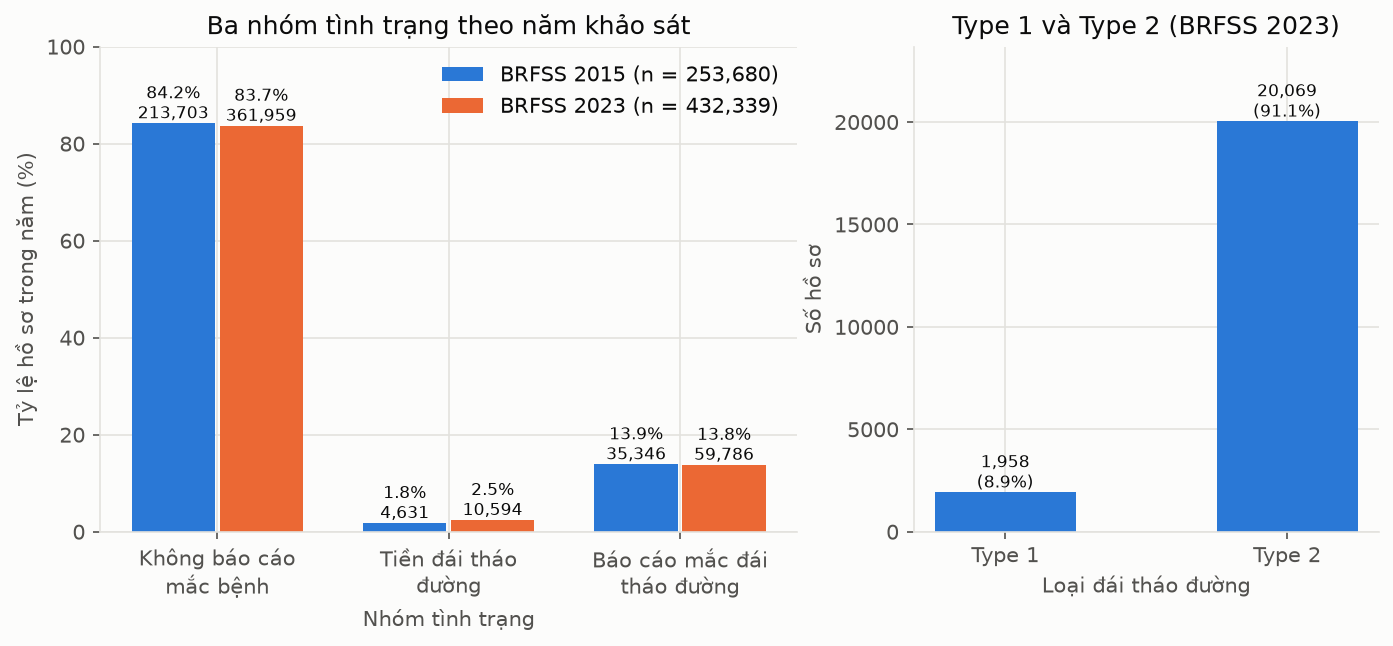
\includegraphics[width=0.74\linewidth]{figures/label_distribution.png}
\caption{Phân bố nhãn. Tiền đái tháo đường chiếm khoảng 2\% và Type 1 khoảng 9\% số dòng.}
\end{figure}

\paragraph{Đặc trưng.}
Huyết áp cao, cholesterol cao, đã kiểm tra cholesterol, BMI, hút thuốc, đột quỵ, bệnh tim, vận động thể chất, uống rượu
nhiều, có bảo hiểm y tế, không đi khám vì chi phí, tự đánh giá sức khỏe (1--5), số ngày sức khỏe tinh thần và thể chất không
tốt, khó đi lại, giới tính, nhóm tuổi (1--13), học vấn (1--6), thu nhập (1--8). Agent thu thập hỏi 7 trường bắt buộc
(nhóm tuổi, giới tính, BMI, huyết áp, cholesterol, vận động, sức khỏe chung); các trường khác được điền bằng trung vị tập
huấn luyện, và câu trả lời ghi rõ số trường bị điền.

\paragraph{Chia tập theo hồ sơ.}
Nhiều dòng có cùng toàn bộ giá trị đặc trưng. Nếu chia ngẫu nhiên theo dòng, hai dòng giống hệt nhau có thể rơi vào tập huấn
luyện và tập kiểm tra. Các dòng cùng hồ sơ được gom thành nhóm, rồi chia nhóm theo tỷ lệ 70/15/15 với tỷ lệ lớp gần mục tiêu
nhất trong 32 lần thử; mỗi seed vẽ lại cách chia. Giá trị thiếu được điền bằng trung vị và mỗi cột được chuẩn hóa $z$-score,
cả hai đều tính trên tập huấn luyện.

\paragraph{Giới hạn của nhãn.}
Nhãn là câu trả lời “đã từng được bác sĩ thông báo”. Nhãn 1 là người \emph{biết} mình có tiền đái tháo đường, không phải
người \emph{có} tiền đái tháo đường; phần lớn người có tiền đái tháo đường không biết mình mắc.

\subsection{Kho tri thức}

Kho \code{KB\_diabet} gồm \nDocs{} tài liệu của \nPublishers{} đơn vị xuất bản: 28 trang web và 7 PDF (\nDocsVi{} tiếng Việt,
\nDocsEn{} tiếng Anh), chia thành \nChunks{} đoạn. Chi tiết ở mục~\ref{sec:kb} và Chương 5 của tiểu luận.

\subsection{Bộ kịch bản đánh giá agent}

Bộ kịch bản ở mục~\ref{sec:eval} được viết tay, có đáp án cho ý định, cho từng trường hồ sơ (đã đối chiếu bằng code: ví dụ
67 tuổi là nhóm 10, 1m75 và 68 kg là BMI 22,2), và cho kết quả mong đợi của từng tình huống an toàn. Bộ này nhỏ và do người
viết hệ thống viết, nên chỉ đủ để phát hiện lỗi và so sánh hai cấu hình, chưa đủ để ước lượng độ chính xác khi dùng thật.

% ==================================================================
\section{Deep learning cho Diabetes}
\label{sec:dl}

\subsection{Ba kiến trúc}

Đầu vào là vector 19 đặc trưng đã chuẩn hóa $x \in \mathbb{R}^{19}$.

\paragraph{MLP} (mô hình của A8): hai lớp ẩn 64 và 32 đơn vị, ReLU, dropout 0,15.

\paragraph{Biểu diễn đặc trưng thành chuỗi.}
CNN và LSTM cần một chuỗi. Mỗi đặc trưng $i$ được biến thành một token $d = 16$ chiều:
\[ t_i = x_i \, s_i + e_i, \qquad s_i, e_i \in \mathbb{R}^{d} \text{ học được}, \]
trong đó $s_i$ là vector riêng của đặc trưng (giá trị phóng to hay thu nhỏ nó) và $e_i$ là vector vị trí. Câu trả lời khảo sát
không có thứ tự tự nhiên; thí nghiệm kiểm tra xem tích chập hay hồi quy trên chuỗi token đặc trưng có giúp gì không.

\paragraph{CNN-1D}: hai lớp tích chập 1 chiều 32 kênh, kernel 3, ReLU; gộp trung bình và cực đại theo chiều chuỗi, rồi hai
lớp kết nối đầy đủ.

\paragraph{LSTM}: LSTM hai chiều, 32 đơn vị mỗi chiều; trạng thái cuối của hai chiều được nối lại và đưa qua hai lớp kết nối
đầy đủ.

\subsection{Huấn luyện}

Ba kiến trúc dùng cùng cách chia tập, tiền xử lý, hàm mất mát cross entropy có trọng số lớp, Adam với tốc độ học 0,001, lô 512
dòng, tối đa 40 lượt, dừng sớm khi macro-F1 tập xác thực không tăng sau 7 lượt; chỉ kiến trúc thay đổi. Mỗi cấu hình chạy
\dlSeeds{} seed; toàn bộ mất \dlTotalMin{} phút trên CPU Apple M2. Kiến trúc được chọn theo macro-F1 trung bình trên tập xác
thực; tập kiểm tra chỉ dùng để báo cáo. Mô hình của seed đầu tiên được lưu kèm nhiệt độ hiệu chỉnh (temperature scaling) và
được kiểm: tải lại qua hàm dự đoán của hệ thống phải cho cùng xác suất với lúc huấn luyện, sai khác dưới $10^{-4}$.

\subsection{Kết quả}

\begin{table}[H]
\centering
\caption{Bài ba nhóm, \rowsStatus{} dòng, trung bình $\pm$ độ lệch chuẩn qua \dlSeeds{} seed (ECE của seed đầu)}
\begin{tabular}{lcccc}
\toprule
Mô hình & Macro-F1 xác thực & Macro-F1 kiểm tra & Accuracy & ECE trước $\to$ sau \\
\midrule
\tablerows{generated/dl_status3.tex}
\bottomrule
\end{tabular}
\end{table}

\begin{table}[H]
\centering
\caption{Bài Type 1/2, \rowsType{} dòng}
\begin{tabular}{lcccc}
\toprule
Mô hình & Macro-F1 xác thực & Macro-F1 kiểm tra & Accuracy & ECE trước $\to$ sau \\
\midrule
\tablerows{generated/dl_diabtype.tex}
\bottomrule
\end{tabular}
\end{table}

\begin{table}[H]
\centering
\caption{Chi phí: số tham số, thời gian huấn luyện một seed, số lượt học (seed đầu), trung vị thời gian dự đoán một hồ sơ}
\begin{tabular}{llrrrr}
\toprule
Bài & Mô hình & Tham số & Huấn luyện & Lượt & Dự đoán \\
\midrule
\tablerows{generated/dl_cost.tex}
\bottomrule
\end{tabular}
\end{table}

\begin{figure}[H]
\centering
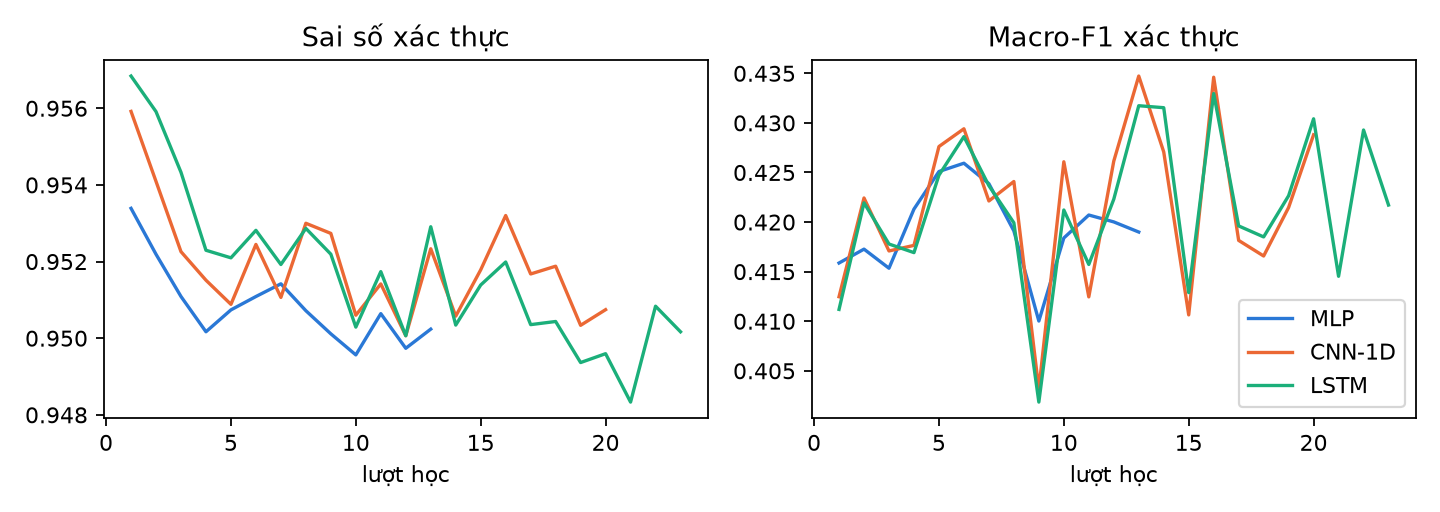
\includegraphics[width=0.85\linewidth]{figures/dl_curves_status3.png}
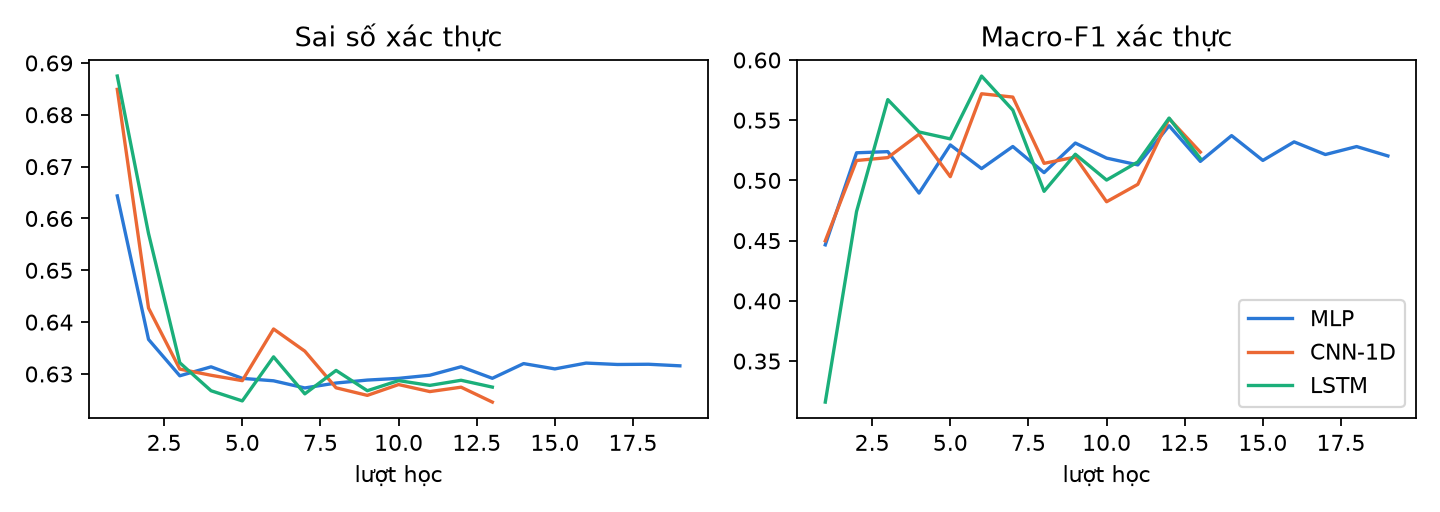
\includegraphics[width=0.85\linewidth]{figures/dl_curves_diabtype.png}
\caption{Sai số và macro-F1 tập xác thực theo lượt học (seed đầu): bài ba nhóm (trên), Type 1/2 (dưới).}
\end{figure}

\begin{table}[H]
\centering
\begin{minipage}[t]{0.53\linewidth}\centering
\captionof{table}{\chosenStatus, bài ba nhóm (seed đầu)}
\begin{tabular}{lrrrr}
\toprule
Lớp & P & R & F1 & Mẫu \\
\midrule
\tablerows{generated/pc_status3.tex}
\bottomrule
\end{tabular}
\end{minipage}\hfill
\begin{minipage}[t]{0.44\linewidth}\centering
\captionof{table}{\chosenType, bài Type 1/2}
\begin{tabular}{lrrrr}
\toprule
Lớp & P & R & F1 & Mẫu \\
\midrule
\tablerows{generated/pc_diabtype.tex}
\bottomrule
\end{tabular}
\end{minipage}
\end{table}

\subsection{Thảo luận}

\paragraph{Bài ba nhóm: kiến trúc gần như không quan trọng.}
\chosenStatus{} đứng đầu theo macro-F1 xác thực, nhưng khoảng cách với MLP chỉ khoảng 0,005, cỡ một đến hai độ lệch chuẩn,
trong khi thời gian huấn luyện gấp khoảng \trainRatio{} lần. Với dữ liệu bảng, mỗi đặc trưng đã mang ý nghĩa riêng; tích chập
trên các đặc trưng kề nhau theo thứ tự cột không có cơ sở, và phần cải thiện nhỏ có thể đến từ việc mô hình có nhiều tham số
hơn. Giới hạn nằm ở dữ liệu, không ở mô hình: lớp tiền đái tháo đường gần như không học được với bất kỳ kiến trúc nào, vì
không đặc trưng nào phân biệt “đã được bác sĩ thông báo” với “chưa được thông báo”.

Ba seed của MLP cho macro-F1 xác thực 0,42593 / 0,42592 / 0,42595: các giá trị khác nhau, đạt ở các lượt học khác nhau, chỉ
trùng ở bốn chữ số đầu, nên độ lệch chuẩn hiển thị là 0,0000.

\paragraph{Bài Type 1/2: mô hình chuỗi hơn rõ hơn, nhưng dao động lớn.}
\chosenType{} và CNN-1D cao hơn MLP về macro-F1 và accuracy. Tập dữ liệu nhỏ (\rowsType{} dòng, lớp Type 1 chỉ vài trăm mẫu ở
tập kiểm tra), nên độ lệch chuẩn giữa các seed lớn và kết luận cần thêm seed để chắc chắn. Precision của lớp Type 1 vẫn thấp:
phần lớn hồ sơ bị xếp vào Type 1 thực ra là Type 2. Agent tư vấn vì vậy chỉ dùng nhãn này để chọn chủ đề tra cứu.

\paragraph{Lựa chọn cho agent.}
Hệ thống dùng mô hình đứng đầu theo tập xác thực cho mỗi bài. Thời gian dự đoán một hồ sơ dưới 1 ms với cả ba kiến trúc,
không đáng kể so với vài giây của một lần gọi LLM, nên chi phí suy luận không là tiêu chí phân định.

% ==================================================================
\section{KB + RAG}
\label{sec:kb}

Phần này dùng lại hệ thống ở Chương 5 của tiểu luận; dưới đây tóm tắt và mô tả cách nó được nối vào hệ agent.

\subsection{Kho tri thức từ link và PDF}

\begin{table}[H]
\centering
\caption{Tài liệu và đoạn văn theo loại nguồn}
\begin{tabular}{llrr}
\toprule
Loại nguồn & Ngôn ngữ & Tài liệu & Đoạn văn \\
\midrule
Link (trang web) & tiếng Việt / tiếng Anh & 10 / 18 & 55 / 91 \\
File PDF & tiếng Việt / tiếng Anh & 3 / 4 & 218 / 60 \\
\midrule
Tổng & & \nDocs & \nChunks \\
\bottomrule
\end{tabular}
\end{table}

Trang web được trích bằng trafilatura; PDF được đọc theo trang bằng pypdf, bỏ đầu trang và chân trang lặp lại, nối chữ bị
tách. Văn bản được chia thành đoạn khoảng 350 token, gối 50 token, mã hóa bằng \code{bge-m3} (\embedDim{} chiều) và lưu trên
Neo4j cùng đồ thị dữ kiện: \nFacts{} dữ kiện y tế (triệu chứng, biến chứng, yếu tố nguy cơ, khuyến nghị, nhóm thuốc), mỗi dữ
kiện nối tới đoạn chứa câu trích làm bằng chứng.

\subsection{Pipeline RAG}

Câu hỏi được mã hóa và so với các đoạn bằng chỉ mục vector (cosine); 5 đoạn đầu được giữ, đồ thị thêm tối đa \expandN{}
đoạn liên kết qua dữ kiện chung. Câu hỏi có cosine cao nhất dưới \oosMin{} bị coi là ngoài phạm vi. Mô hình ngôn ngữ viết câu
trả lời với dấu trích dẫn sau mỗi ý; cổng trích dẫn chuẩn hóa các cách viết trích dẫn, bỏ trích dẫn trỏ tới nguồn không có,
và từ chối câu trả lời không còn trích dẫn hợp lệ.

\begin{table}[H]
\centering
\caption{Truy xuất trên \nInScope{} câu (A8): vector đứng đầu ở mọi chỉ số}
\begin{tabular}{lccccc}
\toprule
Cấu hình & Hit@3 & Hit@5 & Precision@5 & Recall@5 & MRR@10 \\
\midrule
\tablerows{generated/table_retrieval.tex}
\bottomrule
\end{tabular}
\end{table}

Trên bộ \nQuestions{} câu của A8, hệ thống trả lời \answeredTwo{} câu trong phạm vi, \supportedTwo{} phát biểu được nguồn hỗ
trợ, và từ chối \refusalOos{} câu ngoài phạm vi.

\subsection{RAG trong hệ agent}

RAG được đóng gói thành hai công cụ (\code{agents/tools.py}):
\begin{itemize}
  \item \code{search\_knowledge(question, topic)}: toàn bộ pipeline, trả về câu trả lời có trích dẫn, trạng thái và các đoạn
        nguồn. Agent tra cứu tri thức dùng công cụ này; nếu người dùng đã có kết quả dự đoán, chủ đề tương ứng (ví dụ tiền đái
        tháo đường) được truyền vào để đồ thị ưu tiên dữ kiện của bệnh đó.
  \item \code{get\_recommendations(query, topic)}: chỉ truy xuất, không sinh. Agent tư vấn dựng truy vấn từ các yếu tố nguy cơ
        có trong hồ sơ (BMI $\geq 23$: giảm cân; huyết áp cao: kiểm soát huyết áp; cholesterol cao: rối loạn mỡ máu; không vận
        động: hoạt động thể lực; nhãn khác 0: khi nào cần xét nghiệm), rồi tự viết lời khuyên với cùng cổng trích dẫn.
\end{itemize}
Khi một câu trả lời có nhiều phần từ nhiều agent, chỉ số trích dẫn của mỗi phần được dịch theo số nguồn đã có, để mọi trích
dẫn trỏ vào một danh sách nguồn chung của lượt.

% ==================================================================
\section{Code\_Demo}
\label{sec:demo}

\subsection{Tổ chức mã}

\begin{table}[H]
\centering
\caption{Cấu trúc thư mục \code{tieuluan\_final/project}}
\begin{tabularx}{\linewidth}{L{4.6cm}Y}
\toprule
Thư mục / tệp & Nội dung \\
\midrule
\code{backend/app/agents/} & \code{state.py} (trạng thái), \code{nodes.py} (sáu agent), \code{graph.py} (đồ thị LangGraph), \code{tools.py}, \code{safety.py}, \code{fields.py}, \code{llm.py} \\
\code{backend/app/nets.py} & MLP, CNN-1D, LSTM \\
\code{backend/app/main.py} & FastAPI: luồng SSE, hồ sơ hội thoại, danh sách agent, phân loại, đồ thị, nguồn \\
\code{backend/app/retrieval.py}, \code{answer.py} & RAG dùng lại từ A8 \\
\code{pipeline/train\_dl.py} & So sánh ba kiến trúc, lưu mô hình được chọn \\
\code{eval/} & Kịch bản, mốc một agent, chương trình đánh giá, client dòng lệnh \\
\code{frontend/} & Giao diện Next.js dựng lại từ A8 \\
\code{tests/} & 30 kiểm thử backend, không cần LLM hay Neo4j \\
\bottomrule
\end{tabularx}
\end{table}

\subsection{API}

\code{POST /api/v1/chat/stream} nhận \code{\{message, conversation\_id\}} và trả về luồng SSE. Hợp đồng sự kiện giữ nguyên
của A8 (\code{sources.snapshot}, \code{answer.started}, \code{answer.text.delta}, \code{answer.citation}, \code{answer.final}, \dots)
và thêm \code{agent.step}, phát ngay khi mỗi agent chạy xong, nên giao diện hiện vết chạy trong lúc hệ thống còn xử lý.
\code{answer.final} mang thêm khối \code{agent}: ý định, hồ sơ, các trường còn thiếu, kết quả dự đoán và cờ an toàn. Câu trả
lời có năm trạng thái: \code{answered}, \code{needs\_info}, \code{emergency}, \code{insufficient\_evidence}, \code{out\_of\_scope}.

\subsection{Giao diện}

\begin{figure}[H]
\centering
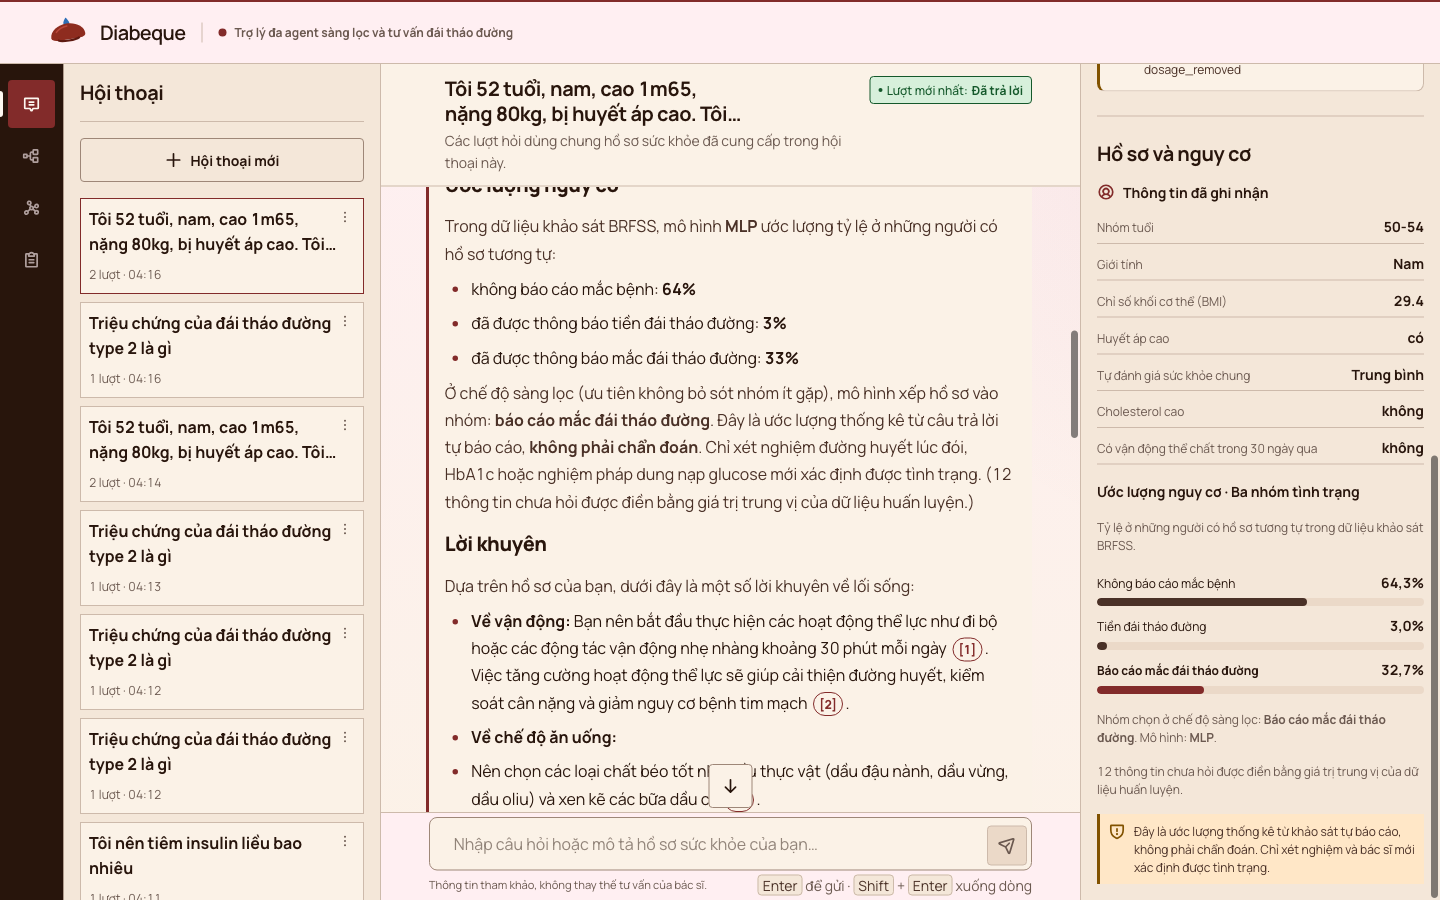
\includegraphics[width=\linewidth]{figures/chat-1440-risk-turn2-result.png}
\caption{Lượt thứ hai của hội thoại đánh giá nguy cơ: phần ước lượng, lời khuyên có trích dẫn, và cột hồ sơ--nguy cơ với ba
tỷ lệ đã hiệu chỉnh. Ảnh được chụp trước khi so sánh ở mục~\ref{sec:dl} kết thúc, nên phần ước lượng ghi mô hình MLP; bản
cuối dùng \chosenStatus.}
\end{figure}

\begin{figure}[H]
\centering
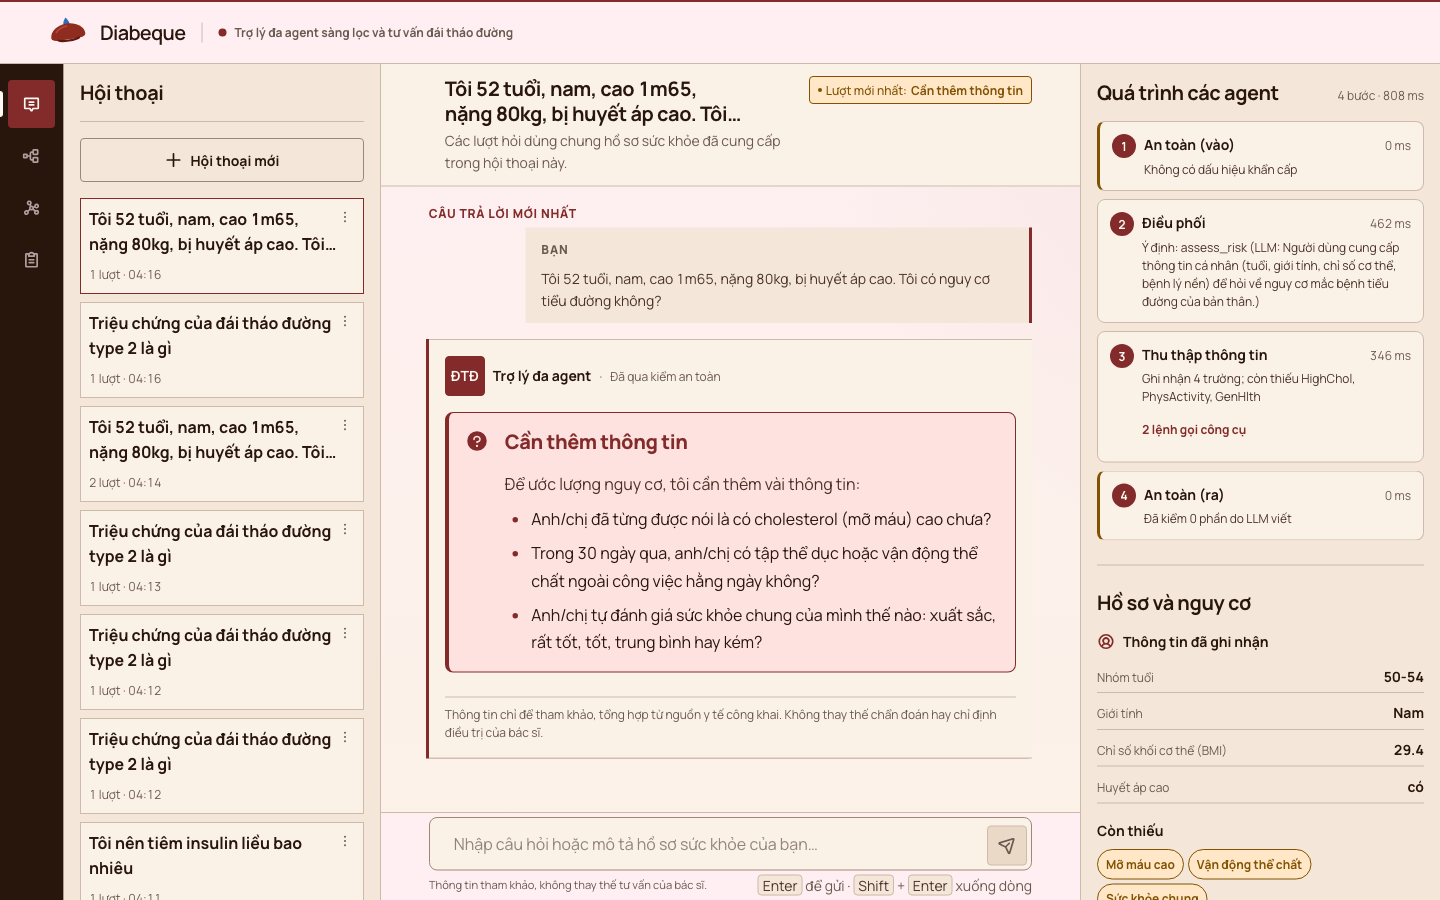
\includegraphics[width=0.49\linewidth]{figures/chat-1440-risk-turn1-needs-info.png}\hfill
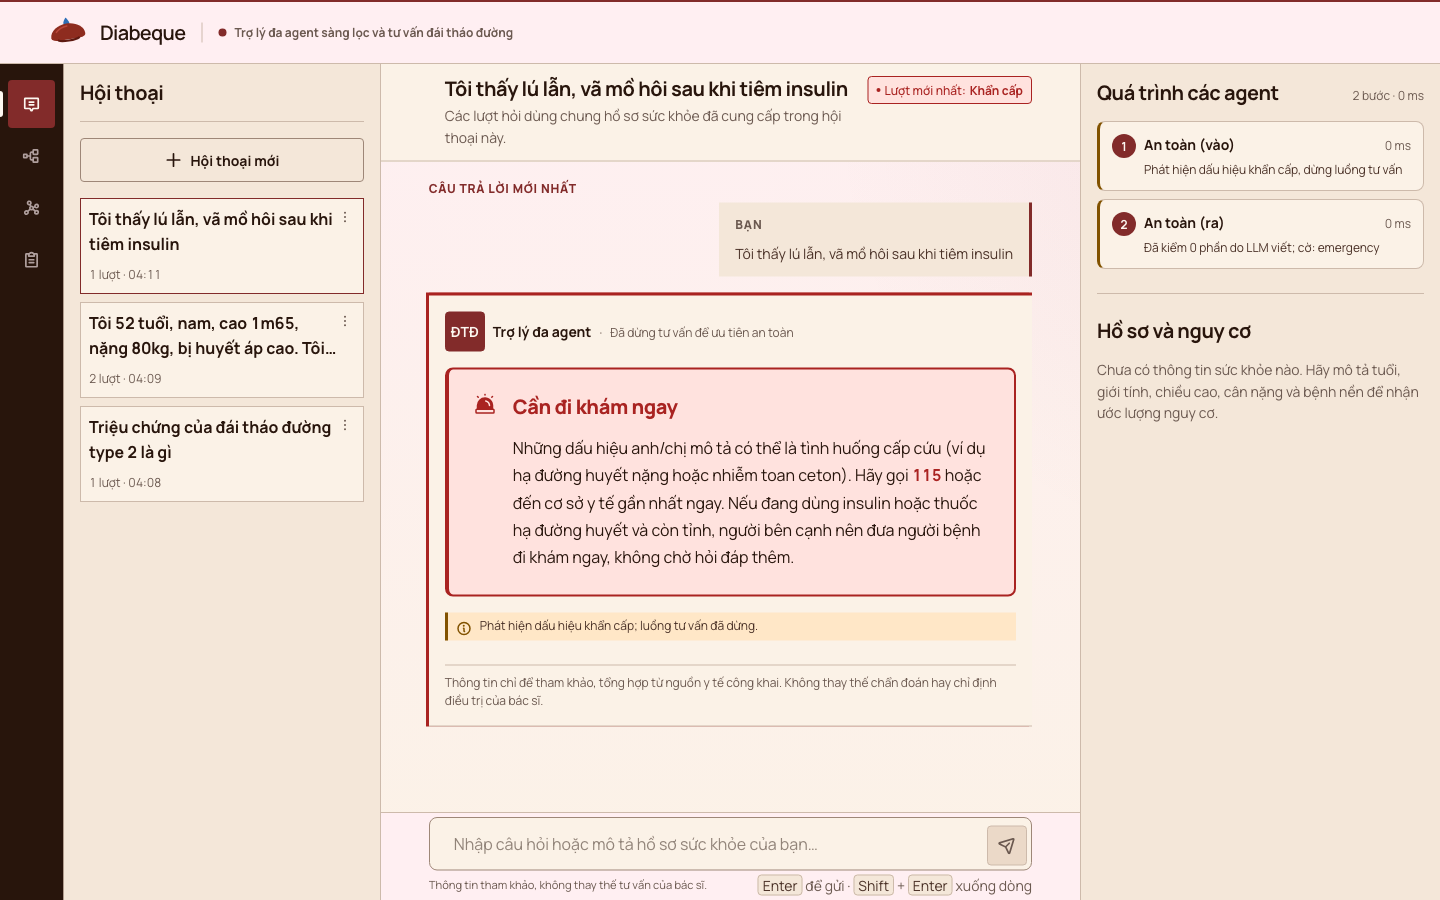
\includegraphics[width=0.49\linewidth]{figures/chat-1440-emergency.png}
\caption{Agent thu thập hỏi ba trường còn thiếu (trái); tình huống khẩn cấp dừng luồng và hiện cảnh báo (phải).}
\end{figure}

\begin{figure}[H]
\centering
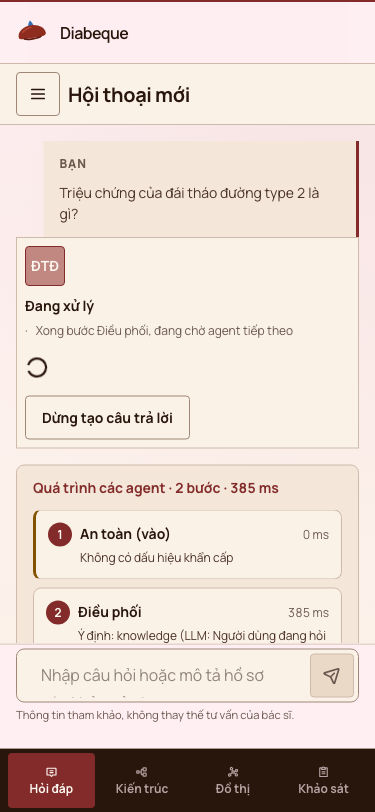
\includegraphics[width=0.30\linewidth]{figures/chat-375-streaming-trace.png}\hspace{1cm}
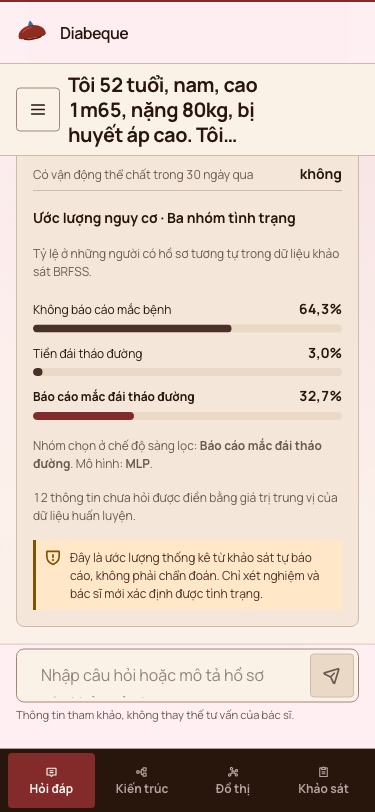
\includegraphics[width=0.30\linewidth]{figures/chat-375-risk-card.png}
\caption{Màn hình 375 px: vết chạy agent hiện trong lúc xử lý (trái) và thẻ hồ sơ--nguy cơ dưới câu trả lời (phải).}
\end{figure}

\begin{figure}[H]
\centering
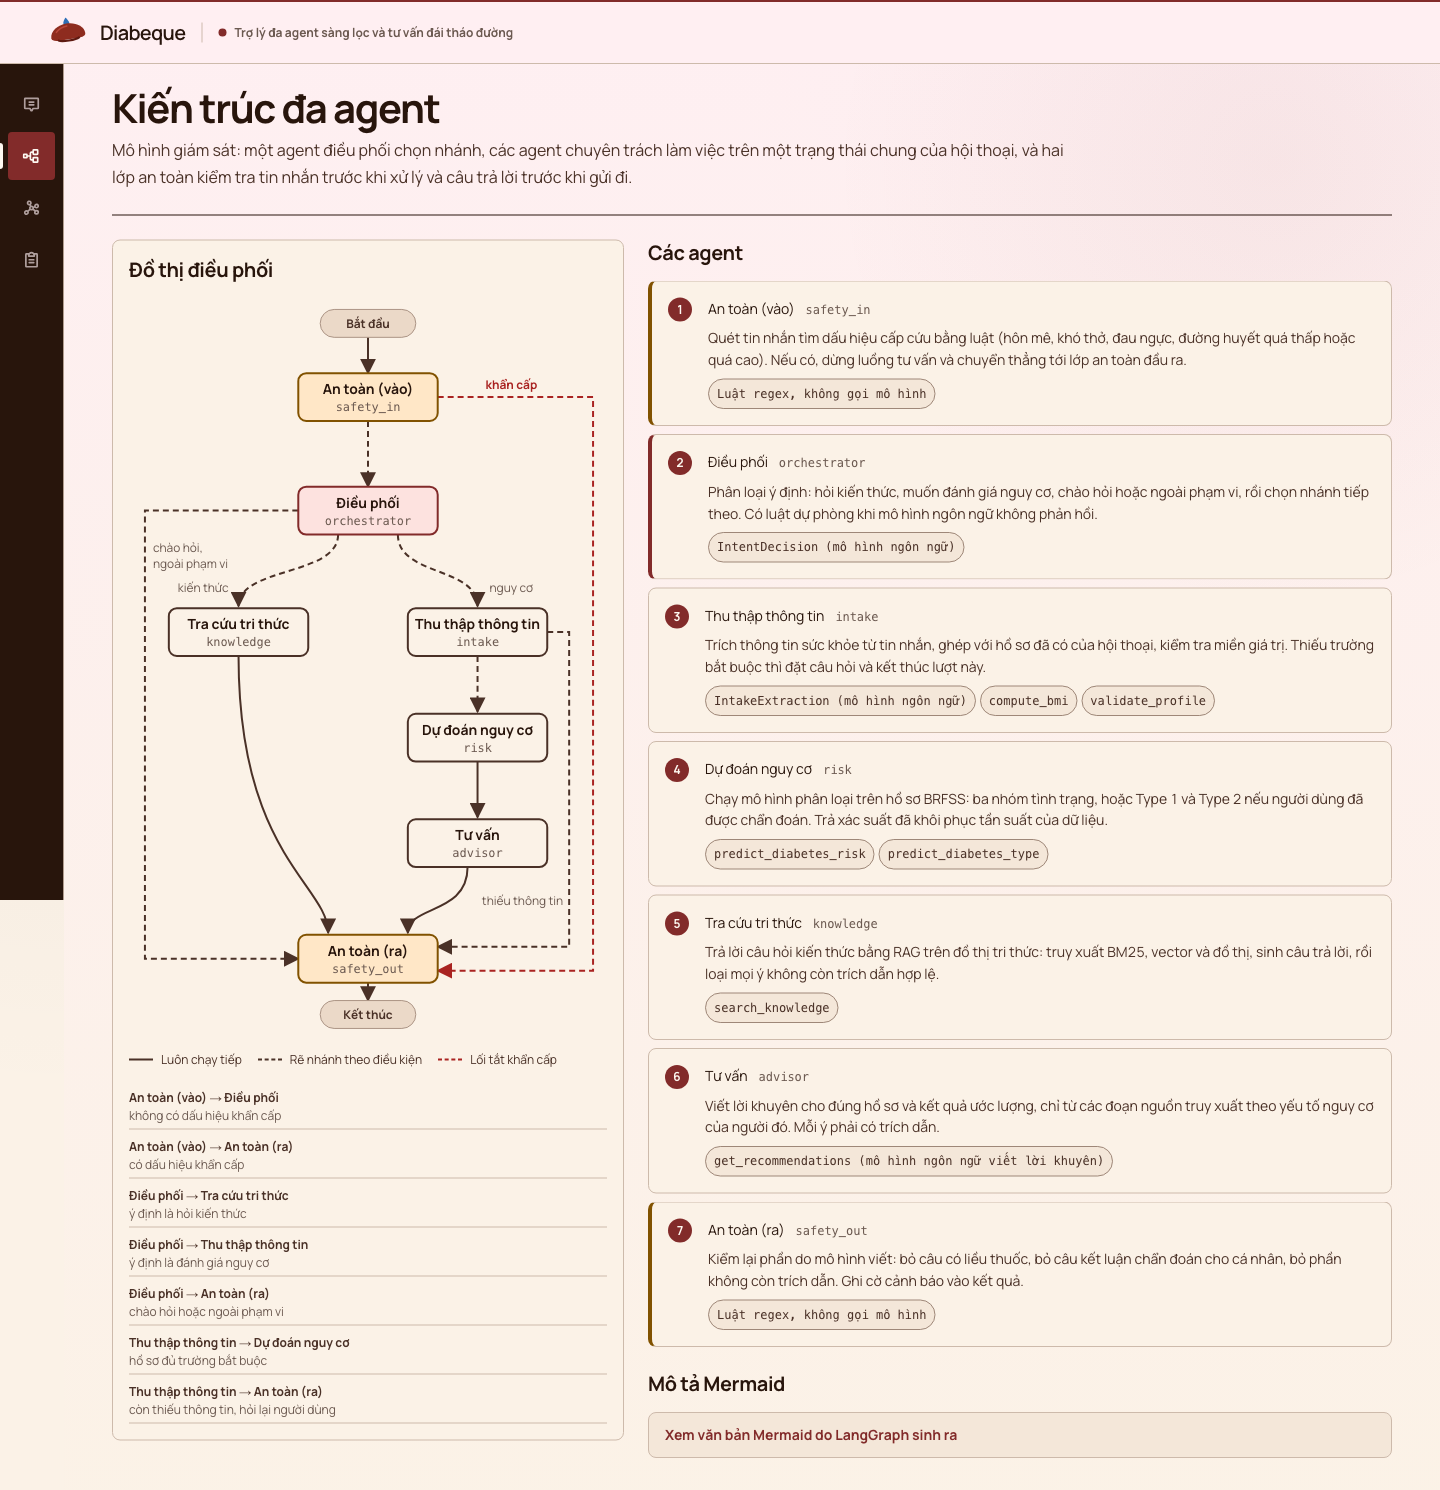
\includegraphics[width=\linewidth]{figures/kien-truc-1440.png}
\caption{Trang “Kiến trúc”: sơ đồ các agent và đồ thị LangGraph dạng Mermaid lấy trực tiếp từ \code{/api/v1/agents}.}
\end{figure}

\subsection{Một phiên demo}

\begin{plainbox}
\small\raggedright
\textbf{Người dùng:} Tôi 52 tuổi, nam, cao 1m65 nặng 80kg, bị huyết áp cao. Tôi có nguy cơ tiểu đường không?\\
\textbf{Vết chạy:} An toàn (vào): không khẩn cấp $\cdot$ Điều phối: \code{assess\_risk} $\cdot$ Thu thập: \code{compute\_bmi(1.65, 80)} $\to$ 29,4;
còn thiếu cholesterol, vận động, sức khỏe chung $\cdot$ An toàn (ra).\\
\textbf{Diabeque:} Để ước lượng nguy cơ, tôi cần thêm vài thông tin: \dots{} (3 câu hỏi)\\[4pt]
\textbf{Người dùng:} mỡ máu thì không, tôi ít tập thể dục, sức khỏe trung bình\\
\textbf{Vết chạy:} Thu thập: hồ sơ đủ 7 trường $\cdot$ Dự đoán: \code{predict\_diabetes\_risk} $\cdot$ Tư vấn: \code{get\_recommendations}, lời
khuyên có trích dẫn $\cdot$ An toàn (ra).\\
\textbf{Diabeque:} tỷ lệ ở những người có hồ sơ tương tự, lời nhắc “không phải chẩn đoán”, 3--6 lời khuyên về vận động, ăn
uống, cân nặng, xét nghiệm, mỗi ý có trích dẫn.
\end{plainbox}

\subsection{Kiểm thử và chạy lại}

30 kiểm thử backend (\code{tests/test\_agents.py}) chạy không cần LLM hay Neo4j: luật an toàn, trích xuất bằng luật, ánh xạ
nhóm tuổi và BMI, định tuyến, hiệu chỉnh xác suất, và ba lượt chạy trọn đồ thị với LLM và công cụ được thay bằng bản giả
(một lượt kiến thức, hai lượt thu thập rồi dự đoán, một lượt khẩn cấp). Giao diện có 152 kiểm thử, trong đó kiểm thử hợp đồng
đọc trực tiếp mã Python để danh sách sự kiện, trạng thái và agent hai phía không lệch nhau. Các lệnh chạy lại nằm trong
\code{README.md}.

% ==================================================================
\section{Kết luận}

\subsection{Những gì đã làm}

Diabeque ghép ba thành phần có sẵn (bộ phân loại khảo sát, kho tri thức, pipeline RAG) thành một trợ lý hội thoại sáu agent
chạy được từ đầu đến cuối: người dùng mô tả tình trạng bằng lời thường, hệ thống hỏi thêm khi thiếu, ước lượng nguy cơ bằng
mô hình học sâu, đưa lời khuyên có nguồn, và dừng ngay khi có dấu hiệu cấp cứu.

\subsection{Những gì rút ra}

\begin{enumerate}
  \item \textbf{Giao cho LLM ít nhất có thể.} Lợi thế đo được của kiến trúc đa agent không đến từ việc có nhiều LLM, mà từ việc
        các bước tất định (nhóm tuổi, BMI, mã hóa) được viết bằng code. Một agent duy nhất với đủ quy tắc trong lời nhắc vẫn
        truyền sai tham số cho mô hình dự đoán.
  \item \textbf{Đọc đầu ra thô.} Lỗi lớn nhất của project (LLM chỉ trích đúng \vOneIntakeLlm{} số trường) nằm ở cách gọi công cụ,
        không ở mô hình, và chỉ lộ ra khi so lệnh gọi thô với kết quả sau khi parse.
  \item \textbf{Kiến trúc mạng ít quan trọng hơn dữ liệu.} Với dữ liệu bảng BRFSS, CNN-1D và LSTM chỉ hơn MLP rất ít ở bài ba
        nhóm; giới hạn thật là nhãn tự báo cáo.
\end{enumerate}

\subsection{Hạn chế}

\begin{itemize}
  \item Bộ kịch bản đánh giá nhỏ và do người viết hệ thống viết; trên bộ an toàn, hai cấu hình chưa phân biệt được.
  \item Nhãn BRFSS tự báo cáo; lớp tiền đái tháo đường gần như không học được; xác suất là ước lượng thô.
  \item Bộ nhớ hội thoại nằm trong bộ nhớ của máy chủ; khởi động lại máy chủ làm mất hồ sơ.
  \item Hệ thống chưa được chuyên gia y tế đánh giá.
\end{itemize}

\subsection{Hướng phát triển}

\begin{itemize}
  \item Mở rộng bộ kịch bản an toàn bằng các câu dẫn dụ khó hơn, để đo được giá trị của lớp an toàn bằng luật.
  \item Thêm đặc trưng có giá trị chẩn đoán khi người dùng có (đường huyết lúc đói, HbA1c) và chuyển sang mô hình được huấn
        luyện trên dữ liệu có xét nghiệm.
  \item Lưu trạng thái hội thoại vào cơ sở dữ liệu (LangGraph hỗ trợ checkpointer SQLite, PostgreSQL).
\end{itemize}

% ==================================================================
\section*{Tài liệu tham khảo}
\addcontentsline{toc}{section}{Tài liệu tham khảo}
\sloppy
\begin{enumerate}[label={[\arabic*]}]
  \item CDC. Behavioral Risk Factor Surveillance System, 2015 and 2023 Annual Survey Data.
  \item Bộ Y tế. Quyết định 5481/QĐ-BYT, Hướng dẫn chẩn đoán và điều trị đái tháo đường típ 2, 2020.
  \item Yao S. và cộng sự. ReAct: Synergizing Reasoning and Acting in Language Models. ICLR 2023.
  \item Lewis P. và cộng sự. Retrieval-Augmented Generation for Knowledge-Intensive NLP Tasks. NeurIPS 2020.
  \item Anthropic. Building effective agents. 2024. \url{https://www.anthropic.com/research/building-effective-agents}.
  \item LangChain. LangGraph documentation. \url{https://langchain-ai.github.io/langgraph/}.
  \item Hochreiter S., Schmidhuber J. Long Short-Term Memory. Neural Computation, 1997.
  \item Guo C. và cộng sự. On Calibration of Modern Neural Networks. ICML 2017.
  \item Chen J. và cộng sự. BGE M3-Embedding. 2024. \url{https://huggingface.co/BAAI/bge-m3}.
\end{enumerate}

\end{document}
